\documentclass[dvipsnames,table,mathserif,aspectratio=169]{beamer} % Definição do tipo de arquivo

\usepackage[T1]{fontenc}      %---------------------------------%
\usepackage[utf8]{inputenc} % Para língua portuguesa          %
\usepackage[brazil]{babel}    %---------------------------------%
\usepackage{times}
\usepackage[export]{adjustbox}
\usepackage{subcaption}

\usepackage[framesassubsections]{beamerprosper} % opções: email, institution,
\usepackage{caption}
\usepackage{stackengine}
\usepackage[portuguese,ruled,lined]{algorithm2e}
\usepackage{algorithmic}
\usepackage{graphicx,url}
\usepackage{enumerate}

\usepackage{amsmath,amsfonts,amsthm,bbm,amssymb}
\usepackage{epsfig}
\usepackage{booktabs}
\usepackage{scalefnt}
\usepackage{commath}

\usepackage{multirow}
% \usepackage[caption=true,font=footnotesize]{subfig}

% \makeatletter
% \patchcmd{\beamer@sectionintoc}
%   {\vfill}
%   {\vskip\itemsep}
%   {}
%   {}
% \makeatother

\captionsetup{compatibility=false}
\newtheorem{myobj}{Objetivos}
\newtheorem{myobjgeral}{Objetivo Geral}
\newtheorem{myobjesp}{Objetivos Específicos}
\usetheme{Execushares}
\newcolumntype{C}[1]{>{\centering\let\newline\\\arraybackslash\hspace{0pt}}m{#1}}


\title[TCC I]{\LARGE{\textbf{Verificação da Autenticidade de Assinaturas Manuscritas Utilizando Redes Neurais Convolucionais}}\\ \ \ \newline \small{Defesa do Trabalho de Conclusão de Curso I}}
\author[Araújo, Guedes]{\textbf{Marcos Wenneton V. de Araujo} \\ Orientadora: Elloá B. Guedes\\\small\email{\{mwvda.eng, ebgcosta\}@uea.edu.br} \\ }
\institute[LSI, EST, UEA]
{
  Grupo de Pesquisa em Sistemas Inteligentes\\
  Escola Superior de Tecnologia\\
  Universidade do Estado do Amazonas\\
  Manaus -- Amazonas -- Brasil
}
\date{\today}


\setcounter{showSlideNumbers}{1}

\AtBeginSection[]
{
  \begin{frame}<beamer>
    \frametitle{Agenda}
    \vskip2\baselineskip            %--------------------------------%
        \fontsize{10}{21}\selectfont% Modificar para caber de acordo %
        \tableofcontents[currentsection]% com a quantidade de seções  %
    \vskip0pt plus 1filll           %--------------------------------%
  \end{frame}
}

\begin{document}
\nocite{*}
\selectlanguage{brazil}

\maketitle

\begin{frame}{Agenda}
  \vskip2\baselineskip            %--------------------------------%
      \fontsize{10}{21}\selectfont% Modificar para caber de acordo %
      \tableofcontents            % com a quantidade de seções     %
  \vskip0pt plus 1filll           %--------------------------------%
\end{frame}

\section{Introdução}

\subsection{Objetivos}

O objetivo geral deste trabalho consiste em verificar a autenticidade de assinaturas manuscritas com redes neurais convolucionais. Para alcançar esta meta, alguns objetivos específicos precisam ser consolidados, a citar:

\begin{enumerate}
  \item Realizar a fundamentação teórica acerca dos conceitos das redes neurais convolucionais;
  \item Consolidar uma base de dados representativa de assinaturas;
  \item Descrever o problema considerado como uma tarefa de Aprendizado de Máquina;
  \item Propor, treinar e testar redes neurais convolucionais para a tarefa considerada;
  \item Analisar os resultados obtidos.
\end{enumerate}

\subsection{Justificativa}

%% Pq resolver esse problema é importante

% Análise de documentos históricos

\subsection{Metodologia}

Para alcançar os objetivos propostos no escopo deste trabalho, a condução das atividades a serem realizadas obedecerá à metodologia descrita a seguir:

\begin{enumerate}
  \item Estudo dos conceitos relacionados ao Aprendizado de Máquinas, Redes Neurais Convolucionais e \emph{Deep Learning};
  \item Descrição do problema considerado como uma tarefa de Aprendizado de Máquina;
  \item Consolidação de uma base de dados representativa de assinaturas originais e forjadas;
  \item Levantamento do ferramental tecnológico para implementação das redes neurais convolucionais;
  \item Proposição de modelos de redes neurais convolucionais para o problema considerado, contemplando arquitetura, parâmetros e hiperparâmetros;
  \item Treino das redes propostas para a tarefa de aprendizado considerada;
  \item Teste das redes previamente treinadas com vistas a coleta de métricas de desempenho;
  \item Análise dos resultados e identificação dos modelos mais adequados para o problema considerado;
  \item Escrita da proposta de Trabalho de Conclusão de Curso;
  \item Defesa da proposta de Trabalho de Conclusão de Curso;
  \item Escrita do Trabalho de Conclusão de Curso; e
  \item Defesa do Trabalho de Conclusão de Curso.
\end{enumerate}

\subsection{Cronograma}

Considerando as atividades enumeradas na metodologia, a Tabela \ref{tab:cronograma} sintetiza o cronograma de execução deste trabalho.

\begin{table}
\scalefont{0.8}
\caption{Cronograma de atividades levando em consideração os dez meses (de $02/2019$ a $12/2019$) para a realização do TCC.}
\label{tab:cronograma}

\begin{center}
\begin{small}
\begin{tabular}{p{5cm}cccccccccccc}
  \toprule
  & &  &  & &  & \textbf{2019}  & &  &  &  &  & \\
                                        & \textbf{02} & \textbf{03} & \textbf{04} & \textbf{05} & \textbf{06} & \textbf{07} & \textbf{08} & \textbf{09} & \textbf{10} & \textbf{11} & \textbf{12} \\
  \midrule

  \textbf{Atividade 1}                     &      X      &      X      &      X      &           &             &             &             &             &             &             &             \\
  \textbf{Atividade 2} &             &      X      &            &             &             &             &             &             &             &             &             \\
  \textbf{Atividade 3}         &             &     X        &    X         &            &            &            &            &            &             &             &             \\
  \textbf{Atividade 4}         &             &             &    X         &            &            &            &            &            &             &             &             \\
  \textbf{Atividade 5}         &             &             &             &      X      &       X     &   X         &     X       &            &             &             &             \\
  \textbf{Atividade 6}         &             &             &             &      X      &     X       &     X       &    X        &            &             &             &             \\
  \textbf{Atividade 7}         &             &             &             &            &            &            &      X      &      X      &             &             &             \\
  \textbf{Atividade 8}         &             &             &             &            &            &            &           &            &   X          &      X       &             \\
  \textbf{Atividade 9}          &      X      &      X      &      X      &      X      &      X      &             &             &             &             &             &             \\

  \textbf{Atividade 10}          &             &             &             &             &      X      &             &             &             &             &             &             \\
  \textbf{Atividade 11}    &             &             &             &             &             &      X      &      X      &      X      &      X      &      X      &      X      \\
  \textbf{Atividade 12}     &             &             &             &             &             &             &             &             &             &             &      X      \\
  \bottomrule
\end{tabular}
\end{small}
\end{center}
\end{table}


\subsection{Organização do Documento}

(..)


\section{Objetivos}
%!TEX root = ../main.tex
\begin{frame}{Objetivos}
	\begin{block}{Objetivo Geral}
	\emph{Verificar a autenticidade de assinaturas manuscritas utilizando Redes Neurais Convolucionais}
	\end{block}
	\pause
	\begin{block}{Objetivos Específicos}
		\begin{itemize}
		\footnotesize
		\item Realizar a fundamentação teórica acerca dos conceitos das redes neurais convolucionais;
		\item Consolidar uma base de dados representativa de assinaturas manuscritas;
		\item Descrever o problema considerado segundo uma tarefa de Aprendizado de Máquina;
		\item Propor, treinar e testar diferentes redes neurais convolucionais para a tarefa considerada;
		\item Analisar os resultados obtidos.
		\end{itemize}
	\end{block}
\end{frame}


\section{Justificativa}
%!TEX root = ../../main.tex


Apesar da capacidade tecnológica atual e da descoberta de uma numerosa quantidade de métodos de biometria, sabe-se que as assinaturas manuscritas ainda possuem papel importante na autenticação de diversos documentos. Justificando, portanto, a necessidade da busca por modelos mais eficientes para a realização da verificação dessas assinaturas.

Como mencionado anteriormente, as assinaturas manuscritas possuem a propriedade de ser pouco invasiva e têm um baixo custo de aquisição. Dessa maneira, a utilização desse método de biometria possui ainda grande relevância atualmente.

Além disso, um problema com a autentificação de identidade de documentos históricos como, por exemplo, quadros, testamentos e cartas importantes que possuem apenas assinaturas manuscritas por pertecerem a épocas onde as tecnologias biométricas não existiam, pode ser facilmente resolvido com os modelos propostos neste trabalho, desde que existam outros documentos com as assinaturas reais dos indivíduos associados aos achados históricos.

No mais, do ponto de vista do bacharel em Engenharia de Computação em formação, a proposta de trabalho de conclusão de curso corrobora para a prática de conceitos, tecnologias e métodos de uma área emergente do Aprendizado de Máquina que é o \emph{Deep Learning}. Por fim, deve-se mencionar a importância da realização deste trabalho com vistas a colaborar com as atividades desenvolvidas pelo \emph{Laboratório de Sistemas Inteligentes} (LSI), uma iniciativa do \emph{Grupo de Pesquisas em Sistemas Inteligentes} da Escola Superior de Tecnologia (EST) da Universidade do Estado do Amazonas (UEA).


%% Pq resolver esse problema é importante

% Análise de documentos históricos
% Método não invasivo de biometria
% Custo baixo da obtenção de Assinaturas
%
% Área emergente Deep learning
% Atividades desenvolvidas pelo LSI


\section{Metodologia}
%!TEX root = ../../main.tex

Para alcançar os objetivos propostos no escopo deste trabalho, a condução das atividades que foram realizadas obedeceram à metodologia descrita a seguir:

\begin{enumerate}
  \item Estudo dos conceitos relacionados ao Aprendizado de Máquinas, Redes Neurais Convolucionais e \emph{Deep Learning};
  \item Descrição do problema considerado como uma tarefa de Aprendizado de Máquina;
  \item Consolidação de uma base de dados representativa de assinaturas originais e forjadas;
  \item Levantamento do ferramental tecnológico para implementação das redes neurais convolucionais;
  \item Proposição de modelos de redes neurais convolucionais para o problema considerado, contemplando arquitetura, parâmetros e hiperparâmetros;
  \item Treino das redes propostas para a tarefa de aprendizado considerada;
  \item Teste das redes previamente treinadas com vistas a coleta de métricas de desempenho;
  \item Análise dos resultados e identificação dos modelos mais adequados para o problema considerado;
  \item Escrita da proposta de Trabalho de Conclusão de Curso;
  \item Defesa da proposta de Trabalho de Conclusão de Curso;
  \item Escrita do Trabalho de Conclusão de Curso; e
  \item Defesa do Trabalho de Conclusão de Curso.
\end{enumerate}


\section{Cronograma}
Considerando as atividades enumeradas na metodologia, a Tabela \ref{tab:cronograma} sintetiza o cronograma de execução deste trabalho.

\begin{table}[h!]
\scalefont{0.8}
\caption{Cronograma de atividades levando em consideração os dez meses (de $02/2019$ a $12/2019$) para a realização do TCC.}
\label{tab:cronograma}

\begin{center}
\begin{small}
\begin{tabular}{p{5cm}cccccccccccc}
  \toprule
  & &  &  & &  & \textbf{2019}  & &  &  &  &  & \\
                                        & \textbf{02} & \textbf{03} & \textbf{04} & \textbf{05} & \textbf{06} & \textbf{07} & \textbf{08} & \textbf{09} & \textbf{10} & \textbf{11} & \textbf{12} \\
  \midrule

  \textbf{Atividade 1}                     &      X      &      X      &      X      &           &             &             &             &             &             &             &             \\
  \textbf{Atividade 2} &             &      X      &            &             &             &             &             &             &             &             &             \\
  \textbf{Atividade 3}         &             &     X        &    X         &            &            &            &            &            &             &             &             \\
  \textbf{Atividade 4}         &             &             &    X         &            &            &            &            &            &             &             &             \\
  \textbf{Atividade 5}         &             &             &             &      X      &       X     &   X         &     X       &            &             &             &             \\
  \textbf{Atividade 6}         &             &             &             &      X      &     X       &     X       &    X        &            &             &             &             \\
  \textbf{Atividade 7}         &             &             &             &            &            &            &      X      &      X      &             &             &             \\
  \textbf{Atividade 8}         &             &             &             &            &            &            &           &            &   X          &      X       &             \\
  \textbf{Atividade 9}          &      X      &      X      &      X      &      X      &      X      &             &             &             &             &             &             \\

  \textbf{Atividade 10}          &             &             &             &             &      X      &             &             &             &             &             &             \\
  \textbf{Atividade 11}    &             &             &             &             &             &      X      &      X      &      X      &      X      &      X      &      X      \\
  \textbf{Atividade 12}     &             &             &             &             &             &             &             &             &             &             &      X      \\
  \bottomrule
\end{tabular}
\end{small}
\end{center}
\end{table}


\section{Fundamentação Teórica}
%!TEX root = ../main.tex


\begin{frame}{Aprendizado de Máquina}
\begin{itemize}
	\item Algoritmos capazes de aprender padrões por meio de exemplos, baseando-se em dados previamente disponíveis
	\bigskip
	\item As técnicas de \alert{Aprendizado de Máquina} têm sido aplicadas com sucesso em um grande número de problemas reais em diversos domínios
	\bigskip
	\item Características: natureza inferencial e a boa capacidade de generalização
	\bigskip
	\item Paradigmas de aprendizado supervisionado e não-supervisionado
\end{itemize}
\end{frame}

\begin{frame}{Redes Neurais Artificiais}
  \vskip2\baselineskip
	\begin{itemize}
		\item Inspiradas na capacidade de processamento de informações do cérebro humano
		\bigskip
		\item \alert{Neurônios artificiais} são as unidades fundamentais de uma RNA
		\item \alert{Função de ativação} fornece a resposta de um neurônio para uma dada entrada
		\bigskip
		\item Neurônios artificiais são conectados entre si na forma de uma rede e distribuídos em uma ou mais camadas ocultas
		\bigskip
		\item Algoritmo \emph{Backpropagation}
		\begin{itemize}
			\footnotesize
			\item Fase \emph{forward} -- produz uma saída para uma dada entrada
			\item Fase \emph{backwards} -- calcula a diferença entre as saídas para minimizar o erro
		\end{itemize}
	\end{itemize}
\end{frame}

\begin{frame}{\emph{Deep Learning} e Redes Neurais Convolucionais}
  \vskip2\baselineskip
\begin{itemize}
	\item \emph{Deep Learning} é uma subárea específica do Aprendizado de Máquina
	\bigskip
	\item Redes Neurais Convolucionais (CNNs):
    \begin{itemize}
      \item Possuem camadas \alert{hierárquicas} e \alert{profundas}
      \item Aproveitam-se da operação matemática denominada \alert{convolução}
      \item Destacam-se pelo reconhecimento de padrões em dados de alta dimensionalidade
    \end{itemize}

    \begin{figure}
    	\caption{Papel das camadas convolucionais e \emph{feature maps} das CNNs}
    	\label{fig:camadas-convolucionais}
    	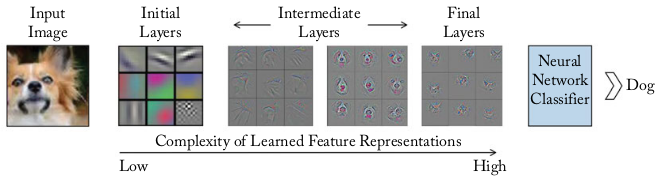
\includegraphics[width=0.5\textwidth]{./img/camadas-convolucionais}
    \end{figure}

\end{itemize}
\end{frame}


\begin{frame}{\Large{Arquiteturas Canônicas de Redes Neurais Convolucionais}}
\begin{itemize}
	\item Arquiteturas com bom desempenho em competições de \alert{Visão Computacional}
	\item Comuns ainda hoje no cenário de \emph{Deep Learning}
	\bigskip
	\item LeNet (1998)
	\item AlexNet (2012)
	\item VGG (2014)
	\item Inception (2014)
	\item ResNet (2015)
\end{itemize}

\end{frame}


\section{Solução Proposta}


\section{Visão Geral do Conjunto de Dados}
% estatisticas calculadas lá no notebook



\section{Preparação do Conjunto de Dados}

\begin{table}[h!]
	\centering
	\caption{Divisão dos dados}
	\label{tab:divisao-dados}
	%\scalefont{0.77}
	\begin{tabular}{c c c c c}
		\toprule
		\textbf{Abordagem} & \textbf{Tipo de Exemplo} & \textbf{Treino} & \textbf{Validação} & \textbf{Teste}\\
		\midrule
		\multirow{2}{*}{1} & genuíno & 2011 & 299 & 618 \\
     & forjado & 11649 & 1648 & 3237 \\
     \midrule
    \multirow{2}{*}{2} & genuíno & 2011 & 299 & 618   \\
     & forjado & 2024 & 308 & 569 \\
		\bottomrule
	\end{tabular}
\end{table}

\begin{figure}[h!]
  \centering
\caption{Visualização da divisão dos dados}
  \subfloat[Abordagem 1\label{subfig:approach1}]{%
    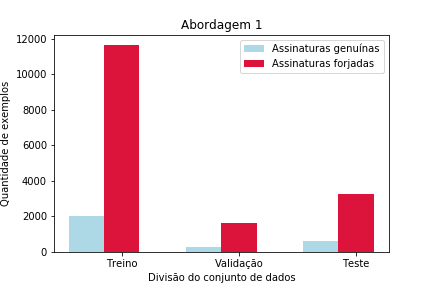
\includegraphics[width=0.7\textwidth]{imgs/approach1}
  }
  \hfill
  \subfloat[Abordagem 2\label{subfig:approach2}]{%
    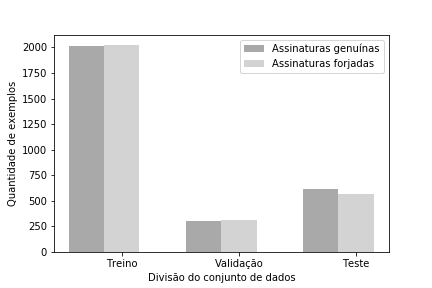
\includegraphics[width=0.7\textwidth]{imgs/approach2}
  }
  \label{fig:divisao-dados}
\end{figure}


\section{Resultados Parciais}
%!TEX root = ../main.tex

Nesta seção serão apresentados os resultados parciais obtidos no teste de modelos baseados em algumas das arquiteturas selecionadas para o escopo deste trabalho. As Seções \ref{sec:lenet} e \ref{sec:alexnet} demonstram os resultados obtidos pelos melhores modelos encontrados com as arquiteturas LeNet e AlexNet, respectivamente. O treinamento destas CNNs foi realizado utilizando os recursos computacionais de um servidor, disponível no LSI, dedicado especialmente para tarefas de DL, o qual possui um processador Intel Core i7 com 16 GB de RAM e duas placas gráficas com 11 GB de memória cada, ajudando no processamento dos algoritmos de aprendizado.

Após a etapa de treino, foram realizados os testes para aferir os modelos no tocante às métricas de desempenho para o conjunto de testes. Nesta etapa, percebeu-se que alguns modelos tornaram-se degenerados e acabaram prevendo apenas uma das classes. Duas hipóteses podem justificar a ocorrência desse problema: o ReLU \emph{dying problem}, quando a função de ativação ReLU foi utilizada; ou a tendência a permanência em mínimos locais durante o treinamento do modelo. Todas as CNNs que manifestaram este comportamento no conjunto de testes tiveram seus resultados descartados, pois as métricas obtidas não refletiam o aprendizado do problema considerado.


\subsection{Resultados Obtidos com a CNN LeNet}
\label{sec:lenet}

A primeira fase do treinamento dos modelos foi conduzida utilizando a arquitetura LeNet. Nesta fase, foi realizada uma busca em \emph{grid} por todos os hiperparâmetros previamente definidos, conforme Seção \ref{sec:modelos}, gerando um total de $36$ modelos a serem treinados e testados. Para estes modelos, excluindo aqueles que se tornaram degenerados, utilizou-se a métrica \emph{F-score} como referência para um melhor desempenho. Em relação aos três otimizadores considerados, os modelos dispostos na Tabela \ref{tab:lenet} foram identificados como tendo melhor desempenho para a tarefa em questão.

\begin{table}[h!]
\centering
\caption{Detalhamento dos melhores modelos obtidos com a arquitetura LeNet, organizados de forma decrescente considerando o valor de acurácia.}
\label{tab:lenet}
\begin{tabular}{ccccc}
\toprule
\textbf{Otimizador} & \textbf{\emph{Patience}}  & \textbf{Função de Ativação} & \textbf{Acurácia} & \textbf{F-Score} \\
\midrule
RMSprop & 5 & \emph{Leaky} ReLU & $0.9865$ & $0.9755$ \\
SGD & 5 & ELU & $0.9787$ & $0.9619$ \\
Adam & 10 & ReLU & $0.9366$ & $0.8974$ \\
\bottomrule
\end{tabular}
\end{table}


Os gráficos da Figura \ref{fig:treinamento-lenet} denotam o histórico da perda (\emph{loss}) e acurácia para o conjunto de treinamento e validação destas redes. Nota-se que nenhuma delas chegou ao limite máximo de épocas possíveis, interrompendo o aprendizado por meio de \emph{early stopping}.


\begin{figure}[h!]
	\centering
	\caption{Histórico de \emph{loss} e acurácia durante o treinamento dos melhores modelos obtidos com a arquitetura LeNet.}
	\subfloat[\emph{Loss} durante treinamento do melhor modelo com RMSprop.\label{subfig:lenet-rmsprop-loss}]{%
	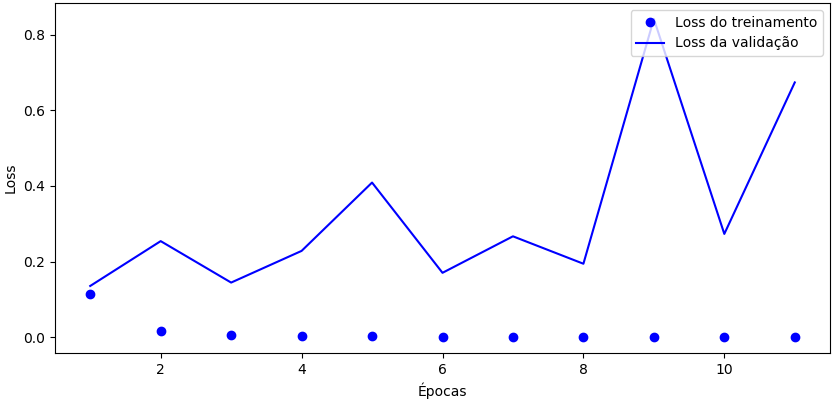
\includegraphics[width=0.45\textwidth]{imgs/lenet-rmsprop-loss}
	}
	\subfloat[Acurácia durante treinamento do melhor modelo com RMSprop.\label{subfig:lenet-rmsprop-acc}]{%
	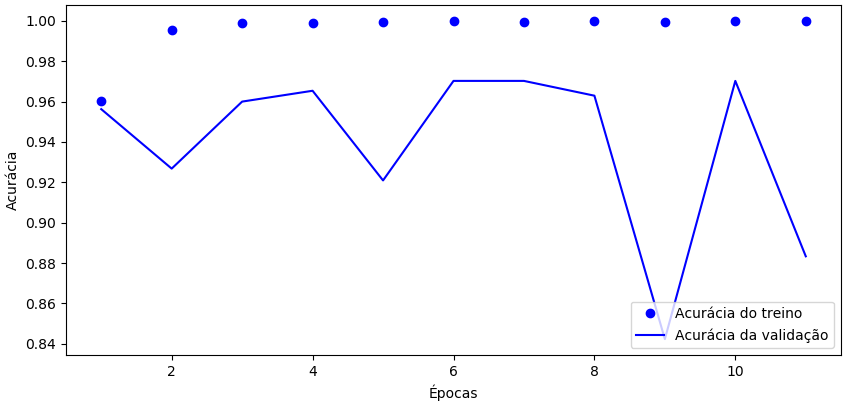
\includegraphics[width=0.45\textwidth]{imgs/lenet-rmsprop-acc}
	}
	\hfill
	\subfloat[\emph{Loss} durante treinamento do melhor modelo com SGD.\label{subfig:lenet-sgd-loss}]{%
	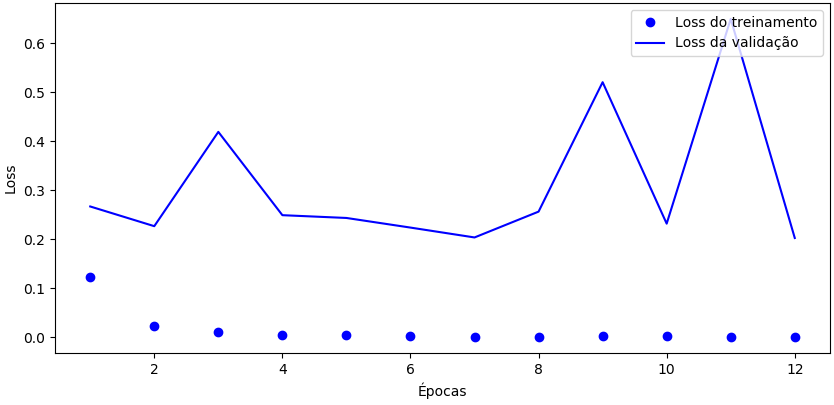
\includegraphics[width=0.45\textwidth]{imgs/lenet-sgd-loss}
	}
	\subfloat[Acurácia durante treinamento do melhor modelo com SGD.\label{subfig:lenet-sgd-acc}]{%
	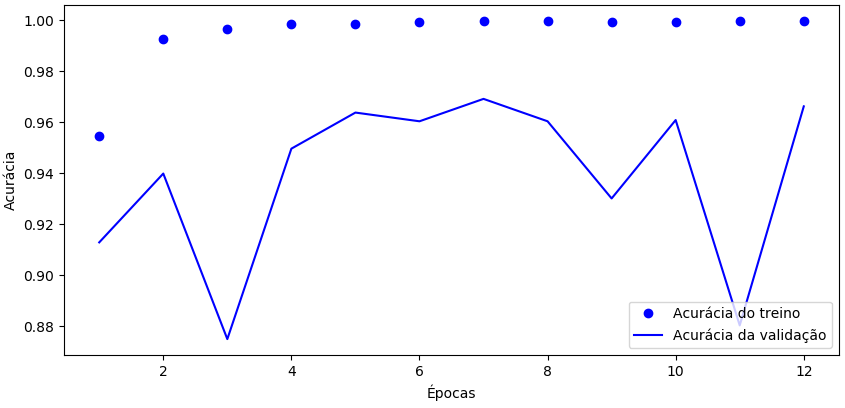
\includegraphics[width=0.45\textwidth]{imgs/lenet-sgd-acc}
	}
	\hfill
	\subfloat[\emph{Loss} durante treinamento do melhor modelo com Adam.\label{subfig:lenet-adam-loss}]{%
	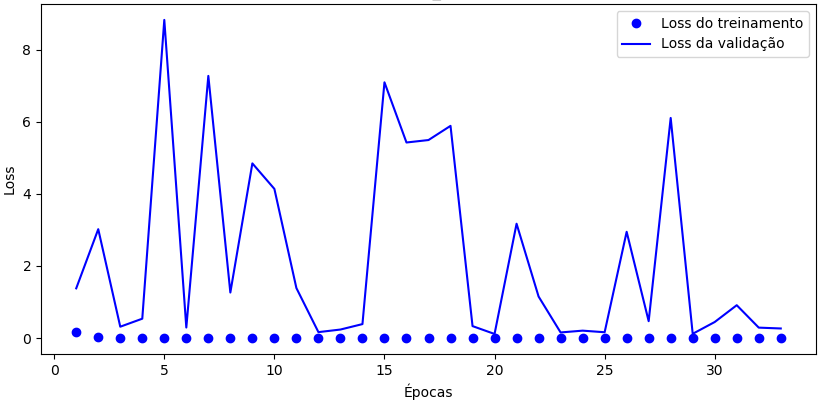
\includegraphics[width=0.45\textwidth]{imgs/lenet-adam-loss}
	}
	\subfloat[Acurácia durante treinamento do melhor modelo com Adam.\label{subfig:lenet-adam-acc}]{%
	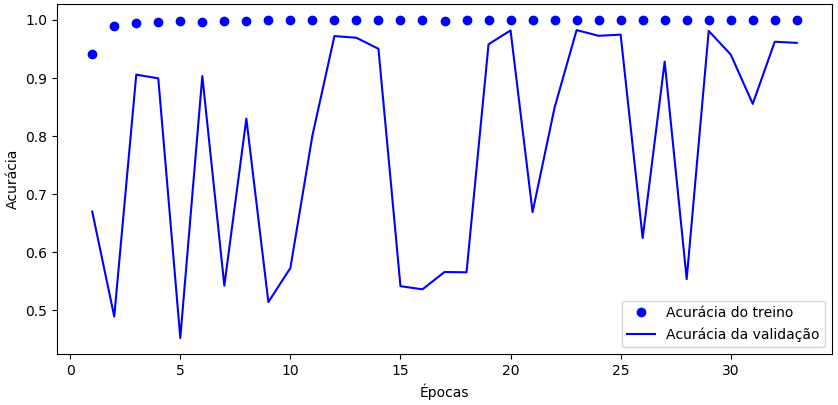
\includegraphics[width=0.45\textwidth]{imgs/lenet-adam-acc}
	}
	\label{fig:treinamento-lenet}
\end{figure}

Examinando mais atentamente o desempenho destas redes no conjunto de testes, tem-se, então, as matrizes de confusão mostradas na Figura \ref{fig:matrizes-lenet}. Nestas matrizes, a soma das linhas representam a quantidade de assinaturas previstas para cada classe pelo modelo em questão, enquanto a soma das colunas denotam a quantidade de assinaturas existentes em cada classe.

\begin{figure}[h!]
	\centering
	\caption{Matrizes de confusão dos melhores modelos obtidos com a arquitetura LeNet.}\label{fig:matrizes-lenet}
	\subfloat[Modelo com RMSprop\label{subfig:matriz-lenet-rmsprop}]{%
	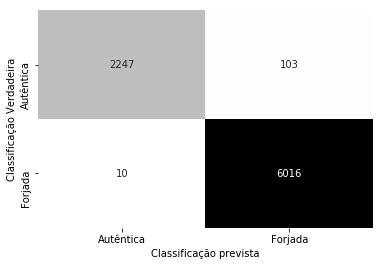
\includegraphics[width=0.5\textwidth]{imgs/matriz-lenet-rmsprop}
	}
	\subfloat[Modelo com SGD\label{subfig:matriz-lenet-sgd}]{%
	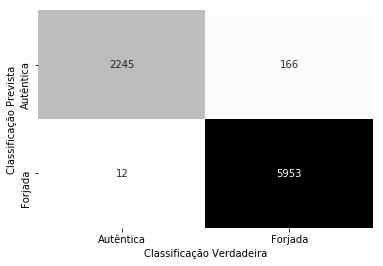
\includegraphics[width=0.5\textwidth]{imgs/matriz-lenet-sgd}
	}
	\hfill
	\subfloat[Modelo com Adam\label{subfig:matriz-lenet-adam}]{%
	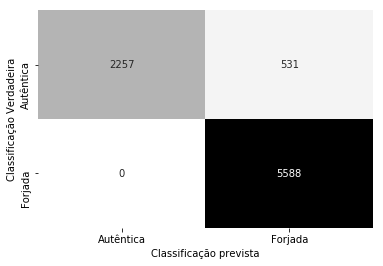
\includegraphics[width=0.5\textwidth]{imgs/matriz-lenet-adam}
	}
\end{figure}

%%%% ARGUMENTAÇÃO

\todo{Refazer a argumentação não se baseando mais nas abordagens}

Para esta arquitetura, é possível visualizar que os melhores modelos foram aqueles que possuíram o menor valor de \emph{patience}. Isso revela que houve uma oscilação no treinamento, de modo que o aprendizado de característica sobre o problema foi instável, resultando em uma parada precoce. Para contornar este efeito, pode ser necessário buscar ajustes de parâmetros (\emph{fine-tuning}) ou também avaliar outras arquiteturas nesta tarefa, nas quais este efeito é minimizado.

No geral, o desempenho obtido com as redes LeNet ainda não foram suficientemente bons para a tarefa considerada. Embora a acurácia denote valores altos para a primeira abordagem ($0.7224$), precisa-se relembrar que isto é mais predominantemente decorrente do desbalanceamento do \emph{dataset} do que da qualidade do modelo em si, conforme revela o \emph{F-Score} associado ($0.1794$). As matrizes de confusão ilustradas na Figura \ref{fig:matrizes-lenet} denotam uma diagonal principal ainda pouco densa, sugerindo que melhorias na tarefa ainda são necessárias. Neste ponto, tem-se os resultados da Abordagem 2 como sendo melhores para a tarefa considerada.



\subsection{Resultados Obtidos com a CNN AlexNet}
\label{sec:alexnet}
 %% Trabalhar aqui

 Para a AlexNet, assim como para a CNN anterior, foi realizada uma busca em \emph{grid} com os hiperparâmetros selecionados anteriormente, com vistas a obter os melhores modelos para cada abordagem de separação de dados, gerando assim, mais 108 modelos a serem avaliados quanto as suas métricas de desempenho.

 Mais uma vez considerando a métrica de \emph{F-score}, foram selecionados os melhores modelos e estes encontram-se listados na Tabela \ref{tab:alexnet}.

 \begin{table}[h!]
 \centering
 \caption{Detalhamento dos melhores modelos obtidos com a arquitetura AlexNet, organizados de forma decrescente considerando o valor de Acurácia.}
 \label{tab:alexnet}
 \begin{tabular}{ccccc}
 \toprule
 \textbf{Otimizador} & \textbf{\emph{Patience}}  & \textbf{Função de Ativação} & \textbf{Acurácia} & \textbf{F-Score} \\
 \midrule
 Adam & 15 & ELU & $0.9654$ & $0.9393$ \\
 SGD & 10 & \emph{Leaky} ReLU & $0.9601$ & $0.9311$ \\
 RMSprop & 15 & \emph{Leaky} ReLU & $0.9397$ & $0.8975$ \\
 \bottomrule
 \end{tabular}
\end{table}


\begin{figure}[H]
	\centering
	\caption{Histórico de \emph{loss} e acurácia durante o treinamento dos melhores modelos obtidos com a arquitetura AlexNet.}
	\label{fig:treinamento-alexnet}
	\subfloat[\emph{Loss} durante treinamento do melhor modelo com Adam.\label{subfig:alexnet-adam-loss}]{%
	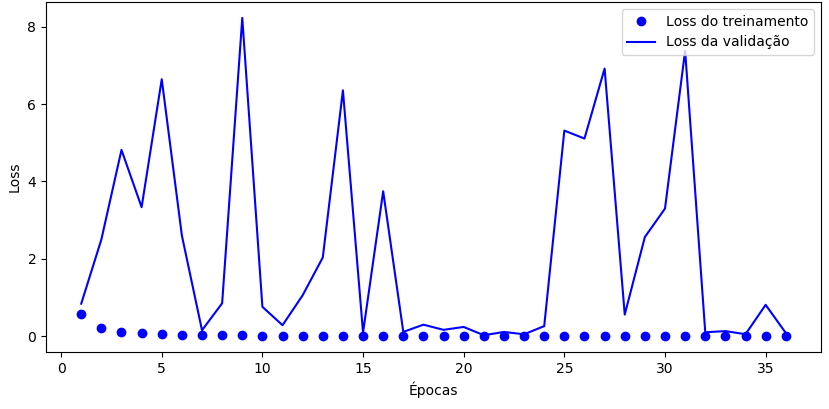
\includegraphics[width=0.45\textwidth]{imgs/alexnet-adam-loss}
	}
	\subfloat[Acurácia durante treinamento do melhor modelo com Adam.\label{subfig:alexnet-adam-acc}]{%
	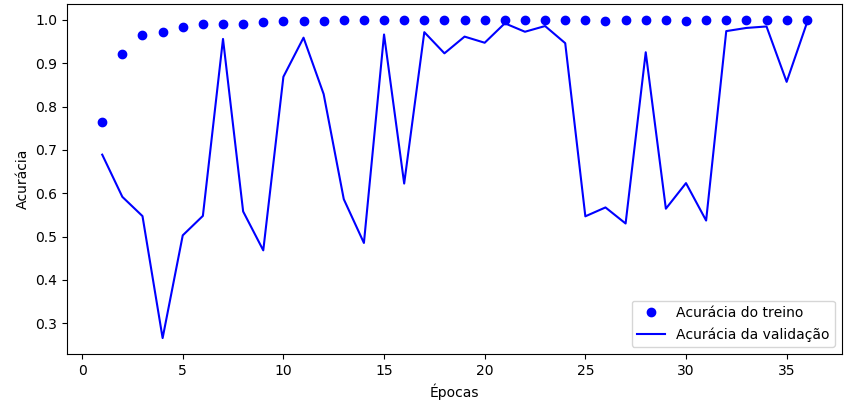
\includegraphics[width=0.45\textwidth]{imgs/alexnet-adam-acc}
	}
	\hfill
	\subfloat[\emph{Loss} durante treinamento do melhor modelo com SGD.\label{subfig:alexnet-sgd-loss}]{%
	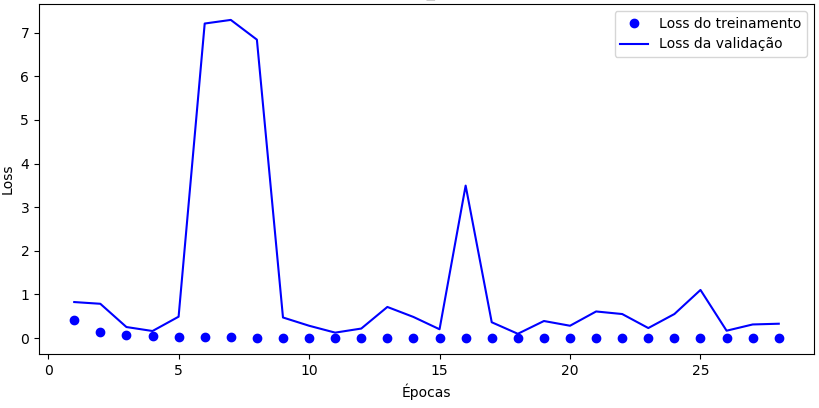
\includegraphics[width=0.45\textwidth]{imgs/alexnet-sgd-loss}
	}
	\subfloat[Acurácia durante treinamento do melhor modelo com SGD.\label{subfig:alexnet-sgd-acc}]{%
	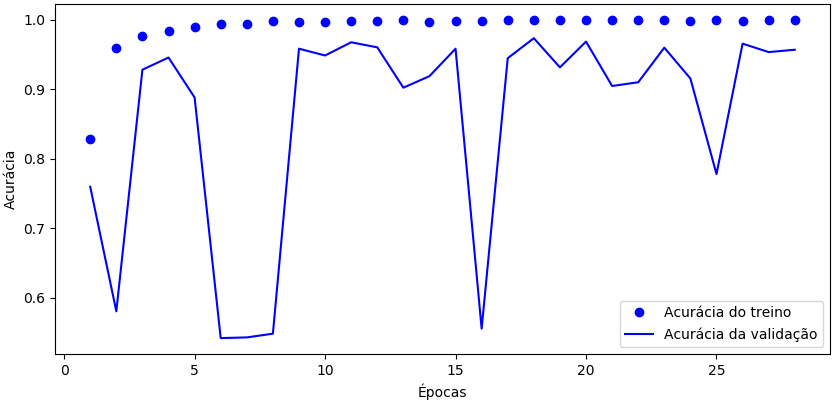
\includegraphics[width=0.45\textwidth]{imgs/alexnet-sgd-acc}
	}
	\hfill
	\subfloat[\emph{Loss} durante treinamento do melhor modelo com RMSprop.\label{subfig:alexnet-rmsprop-loss}]{%
	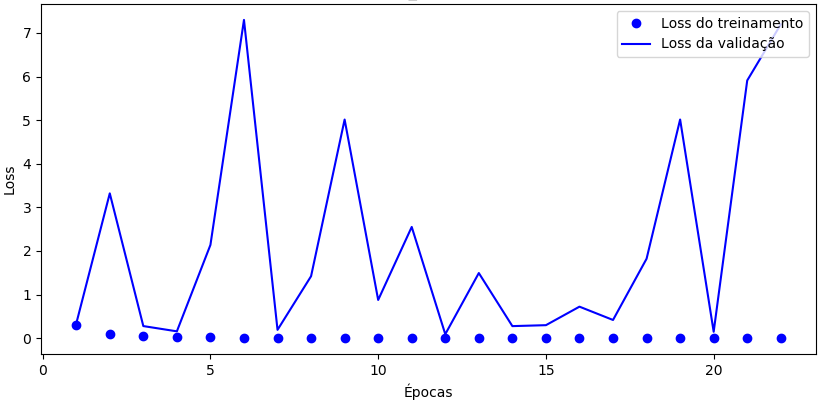
\includegraphics[width=0.45\textwidth]{imgs/alexnet-rmsprop-loss}
	}
	\subfloat[Acurácia durante treinamento do melhor modelo com RMSprop.\label{subfig:alexnet-rmsprop-acc}]{%
	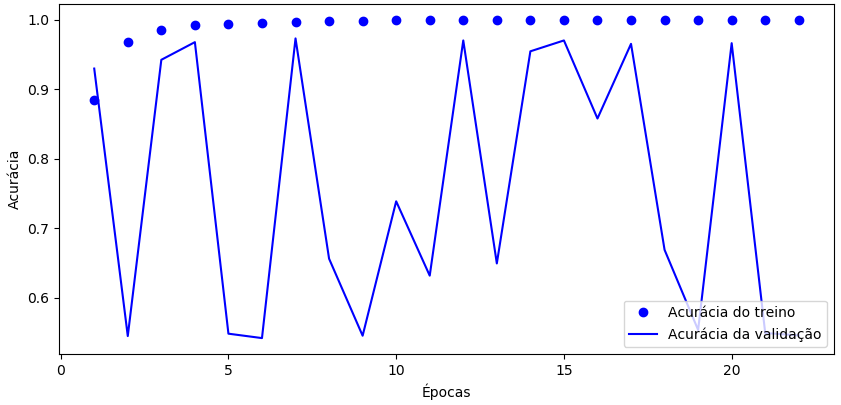
\includegraphics[width=0.45\textwidth]{imgs/alexnet-rmsprop-acc}
	}
\end{figure}


\begin{figure}[H]
	\centering
	\caption{Matrizes de confusão dos melhores modelos obtidos com a arquitetura AlexNet.}
	\subfloat[Modelo com Adam\label{subfig:matriz-alexnet-adam}]{%
	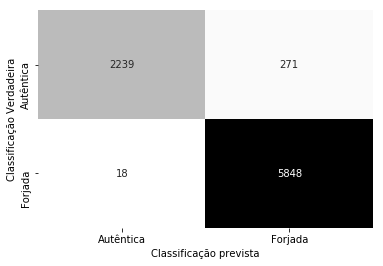
\includegraphics[width=0.5\textwidth]{imgs/matriz-alexnet-adam}
	}
	\subfloat[Modelo com SGD\label{subfig:matriz-alexnet-sgd}]{%
	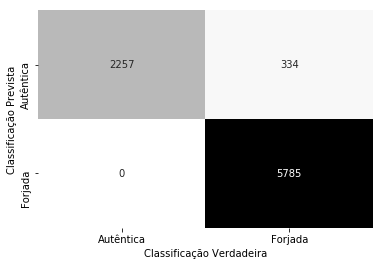
\includegraphics[width=0.5\textwidth]{imgs/matriz-alexnet-sgd}
	}
	\hfill
	\subfloat[Modelo com RMSprop\label{subfig:matriz-alexnet-rmsprop}]{%
	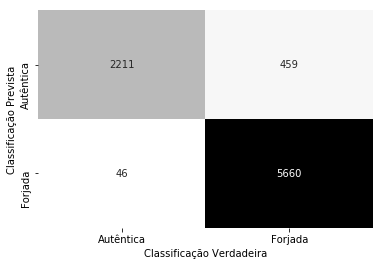
\includegraphics[width=0.5\textwidth]{imgs/matriz-alexnet-rmsprop}
	}
	\label{fig:matrizes-alexnet}
\end{figure}


\section{Considerações Parciais}
%!TEX root = ../main.tex

\chapter{Considerações Finais} \label{cap:consideracoes}

%% Problema, tarefa, o uso de Redes Neurais Convolucionais para abordar esta tarefa e a separação dos dados promovendo uma proximidade com o cenário relatístico
O objetivo desta proposta de trabalho de conclusão de curso consistiu em endereçar o problema de autenticação de assinaturas manuscritas considerando a perspectiva de Aprendizado de Máquina utilizando Redes Neurais Convolucionais. Para isto, foi selecionado um conjunto de dados contendo assinaturas forjadas e genuínas, o qual foi preparado para a tarefa de interesse, contendo $27.962$ exemplos. Estes dados foram particionados em conjuntos de treino, teste e validação com a ressalva de que apenas falsificações inéditas compuseram o conjunto de teste, visando aproximar a avaliação de cenários realísticos. Esta base se de dados foi então utilizada para treinamento e teste de arquiteturas de redes neurais convolucionais bem estabelecidas na literatura.

Dentre as arquiteturas escolhidas, na primeira parte deste trabalho foram consideradas a LeNet e a AlexNet, as quais passaram por uma busca em \emph{grid} que combinou vários valores de hiperparâmetros, culminando no treinamento e teste de um total de $72$ modelos. Dentre estes, aquele que resultou em um melhor desempenho, é caracterizado pela arquitetura LeNet, utiliza o otimizador RMSProp, possui \emph{patience} igual a 5 e utiliza função de ativação \emph{Leaky} ReLU. Este modelo obteve uma acurácia de $98.65\%$ e um valor de \emph{F-score} igual a $0.9755$. Se considerada apenas a habilidade deste modelo em identificar falsificações, ignorando-se os resultados obtidos para assinaturas autênticas, tem-se um \emph{F-Score} igual a $0.9915$ para esta habilidade\footnote{Calculou-se este \emph{F-Score} tomando o valor $6016$ como sendo de verdadeiros positivos e o valor $103$ como sendo de falsos negativos.}. Além do bom desempenho obtido, ressalta-se que esta arquitetura é a que possui menos parâmetros dentre as avalidadas até o momento, o que agrega um valor ainda maior aos resultados obtidos em virtude do menor esforço computacional para realização de previsões e menor espaço em disco para armazenamento. \todo{Rever a necessidade desse páragrafo}

Considerando o bom desempenho já conquistado nesta tarefa e demonstrando a adequação dos modelos para o que foi proposto, tem-se em mente, na próxima etapa deste trabalho, prosseguir primeiramente com topologias que possuam menos parâmetros, em especial, as arquiteturas SqueezeNet e MobileNet. Após isto, será considerada também a avaliação de redes mais profundas, como a VGG-16 e a Inception, possivelmente utilizando técnicas de \emph{Data Augmentation}, se necessário, para contornar as limitações relativas ao tamanho do conjunto de dados disponível.\todo{Rever a necessidade desse páragrafo}

O problema em questão é significativo do ponto de vista prático pois pode colaborar, por exemplo, para a autenticação de documentos de maneira automática e confiável diminuindo os recursos humanos especializados para este fim. Do ponto de vista do bacharel em Engenharia de Computação que desenvolve este trabalho, construir uma solução para este problema foi a oportunidade de pôr em prática diversos conceitos aprendidos ao longo do curso, principalmente aqueles presentes nas disciplinas de Inteligência Artificial, \emph{Machine Learning}, Redes Neurais Artificiais, Linguagem de Programação, Sinais e Sistemas e Processamento Digital de Imagens.


\section{Referências}
%!TEX root = ../main.tex

\begin{frame}{Referências}
\begin{itemize}
\footnotesize
\item BRAGA, A. de P.; CARVALHO, A. P. de Leon F. de; LUDERMIR, T.B. \emph{Redes Neurais Artificiais: Teorias e Aplicações}. Rio de Janeiro, RJ: Livros Técnicos e Científicos Editora S.A., 2000.
\ \ \newline
\item BLANKERS, V. L. et al. \emph{The icdar 2009 signature verification competition}. In: \emph{10th International Conference on Document Analysis and Recognition}. Barcelona, Catalonia, Spain: IEEE, 2009. p. 1403-1407.
\ \ \newline
\item KHAN, S. et. al. \emph{A Guide to Convolutional Neural Networks for Computer Vision}. Austrália: Morgan \& Claypool, 2018.
\ \ \newline
\item LIWICKI, M. \emph{IAPR TC11 - ICDAR 2009 Signature Verification Competition (SigComp2009)}. 2012. Disponível em: hhttp://www.iapr-tc11.org/mediawiki/index.php?title=IAPR-TC11:Reading Systemsi. Acesso em 5 de março de 2019.
\end{itemize}
\end{frame}


\section*{}
\maketitle

\end{document}
